\subsection{Functional description}
	The team is tasked with creating a system that mines social data and curated
traffic information provided from Transport for London, in order to provide
insight into the current state of road traffic.

This system should mine and identify tweets that discuss road traffic for a
particular region. Initially these tweets should be correlated with the TfL
traffic disruptions, but to capture new and evolving events, the inferencing of
traffic disruptions from tweets alone should be investigated.

Practically there should be a user interface to the system that enables the
user to view a list of disruptions each with a useful additional information
and the social conversation surrounding the disruption.



Beginning with the initial project description the team explored a number of
concepts that would potentially fit the project description.

From the description it was clear that a server providing collection of data
from twitter, analysis, processing, storage and retrieval, and a client
providing the user interface to the project were required. Over two team
meetings, system architectures were explored on a whiteboard illustrated in
Figure~\ref{fig:whiteboarding_session}. This firstly was useful as it gave time for
everyone on the team to become comfortable with the project and helped to
identify each of the areas of experience of each person on the team.

\begin{figure}[htb]
\centering
\mbox{\subfigure{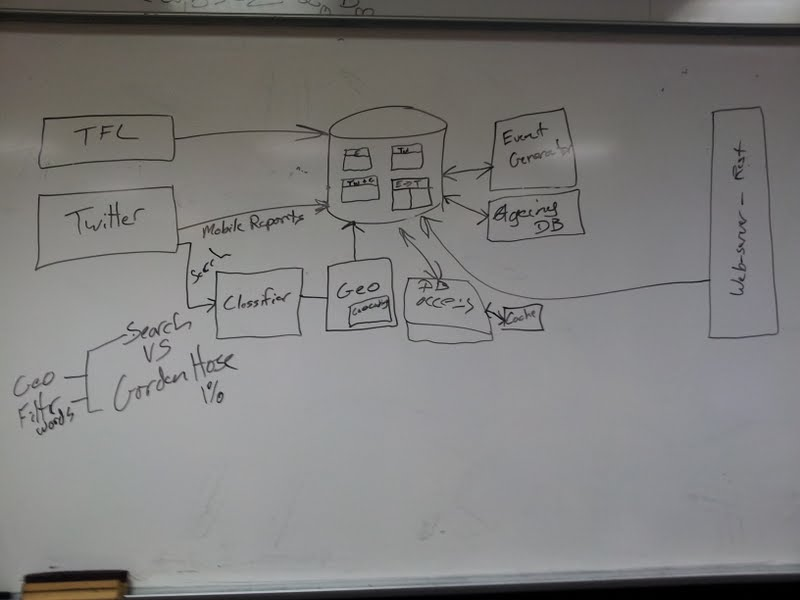
\includegraphics[width=0.4\textwidth]{images/specification/whiteboard_session.jpg}
\quad
\subfigure{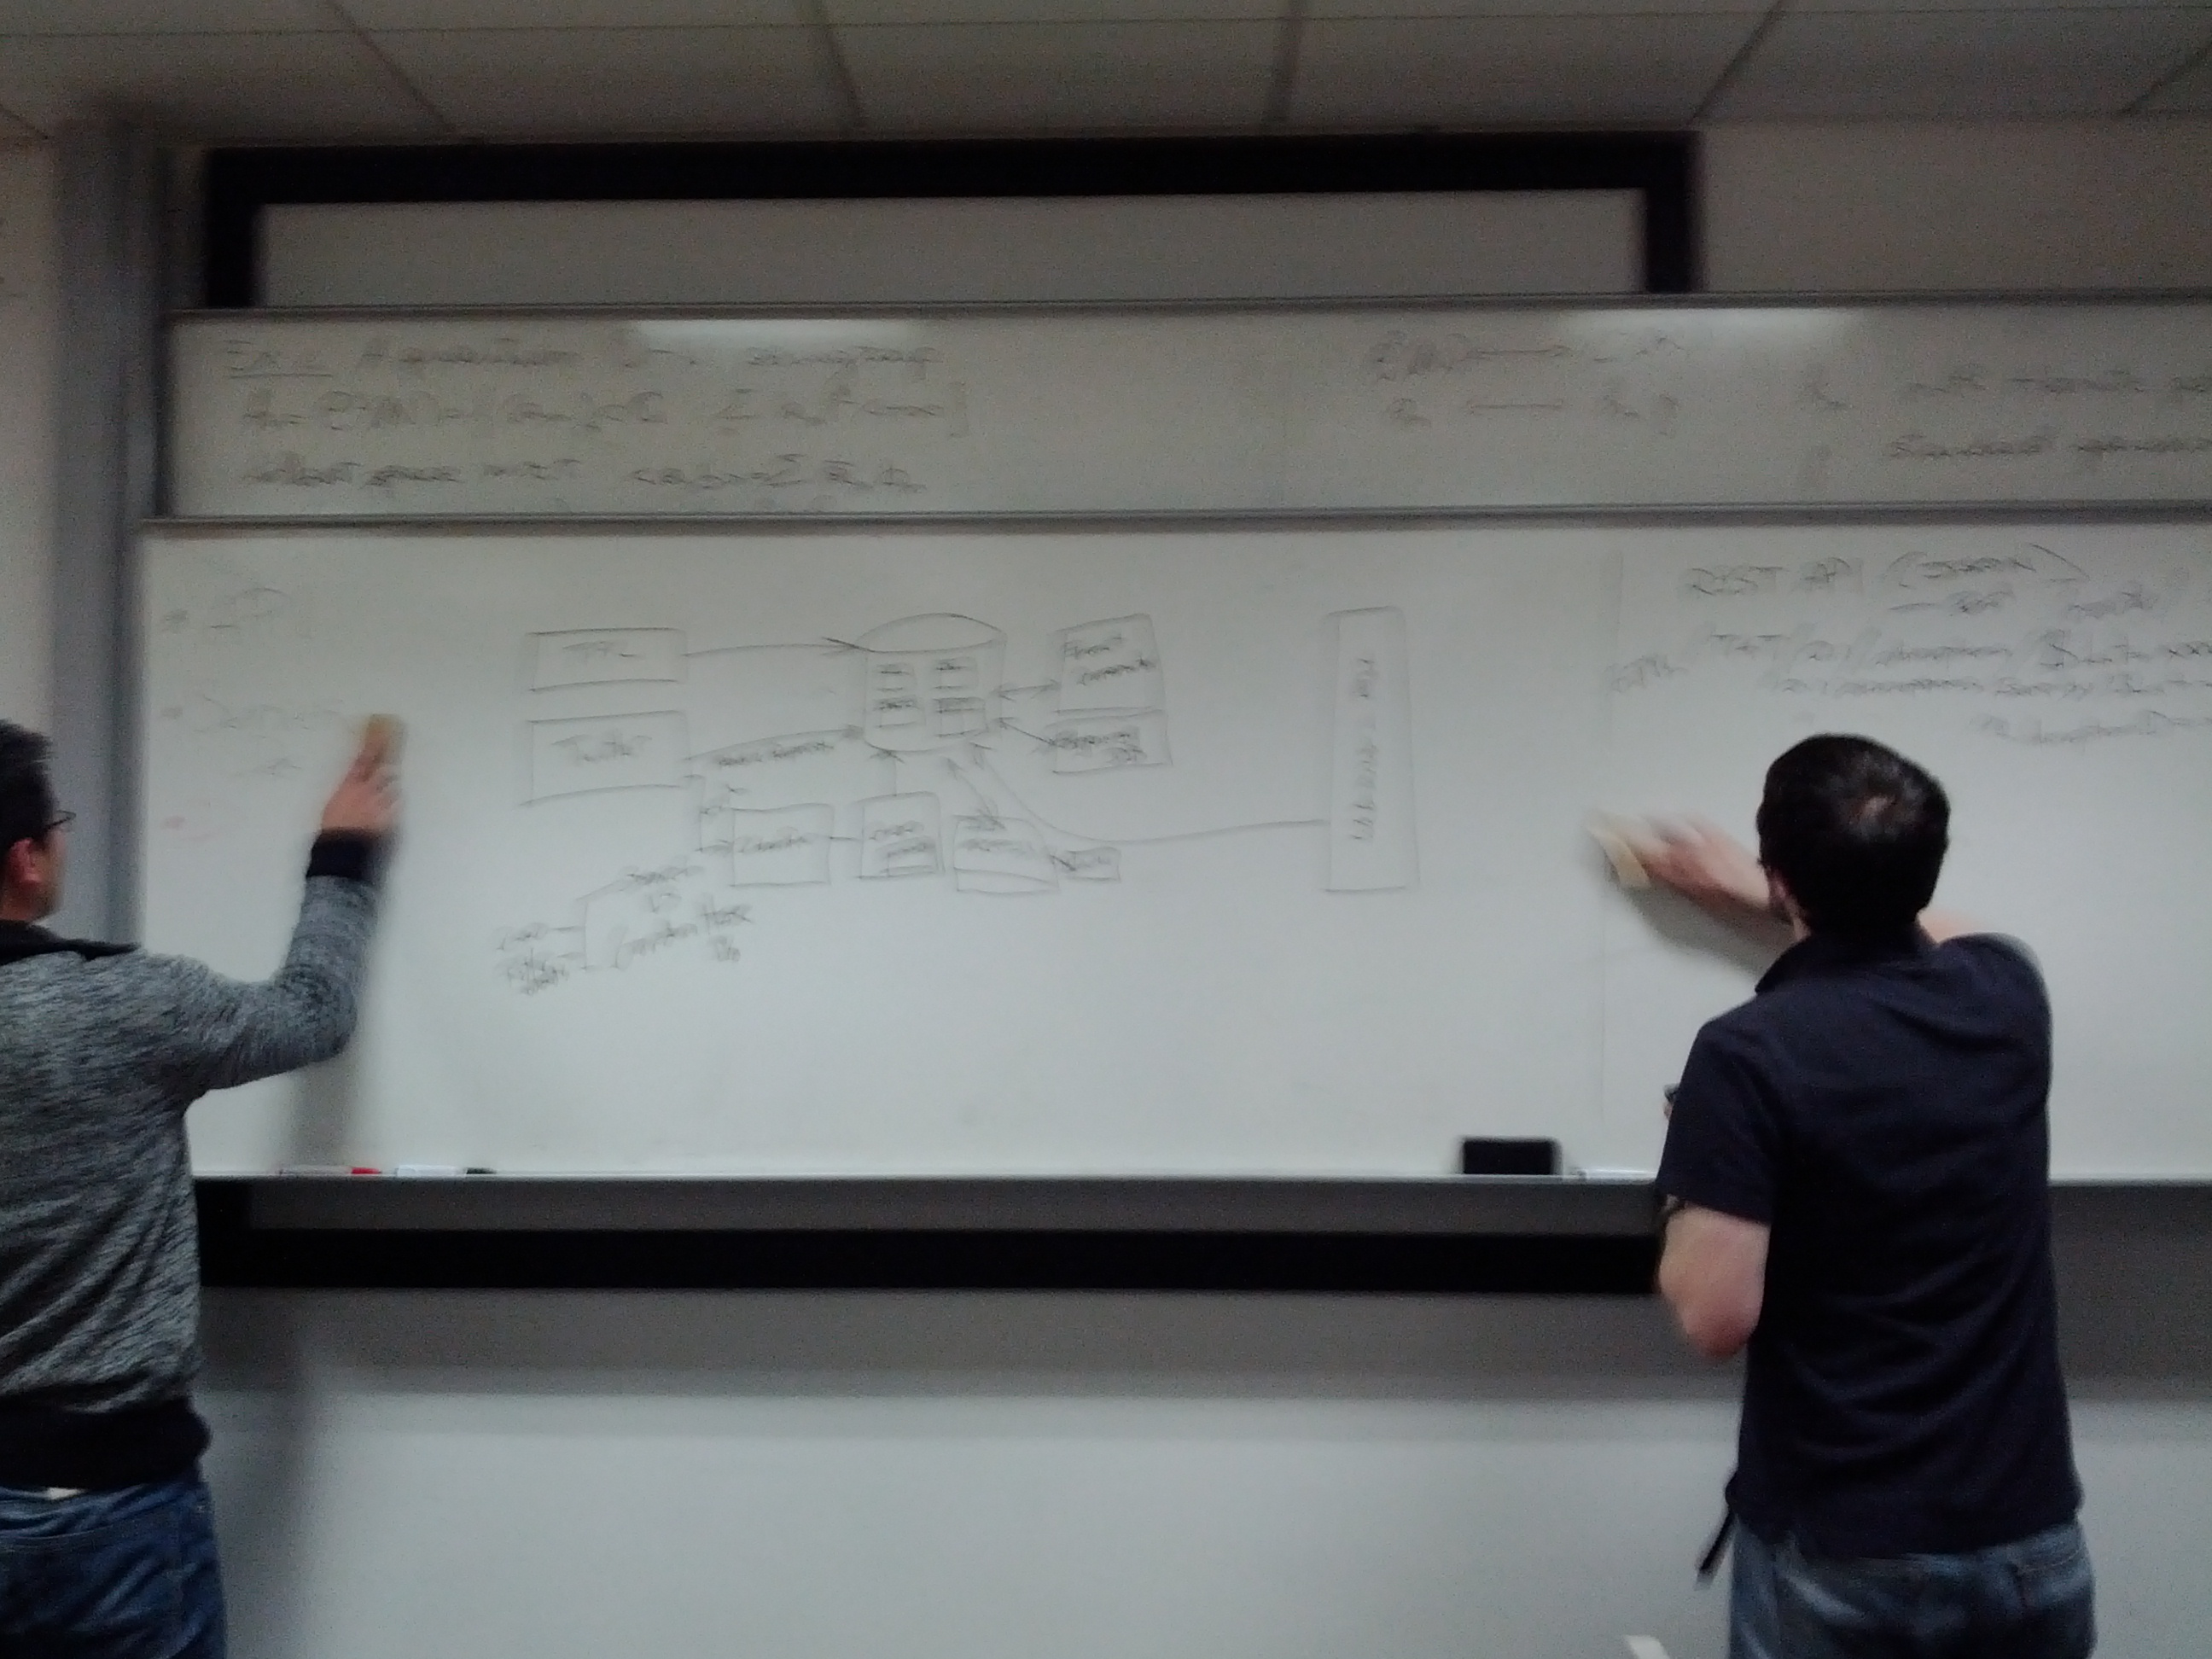
\includegraphics[width=0.4\textwidth]{images/specification/whiteboard_session1.jpg} }}}

\caption{Whiteboarding session}
\label{fig:whiteboarding_session}
\end{figure}

With this conceptual architecture in the requirements for the project were
identified using goal-orientated capture \cite{dardenne93}. The requirements were validated by
the project supervisors and a number of small improvements were suggested.

All the requirements and features were assigned into the two major components of the system, 
the Client and the Server. The features are described in seperate tables according to which component they belong. 
Additionally, the priority and feasibility measures are listed for each feature, using metrics from 
1 to 10, with 1 being the most important feature(priority) or the easiest to implement(feasibility). 
The last column indicates if the current feature has been successfully completed or not. The reasons for 
not completing them are specified in a later section of the report.

\subsection{Server}

\begin{center}
\begin{tabular}{ | p{8.5cm} | c | c | c | }
\hline
\multicolumn{4}{|c|}{\textbf{Server Application}} \\ \hline
\textbf{Feature} & \textbf{Priority} & \textbf{Feasibility} & \textbf{Completed}
\\ \hline
\textbf{Store disruptions from TfL} \newline
Create a geographic database of live events from TfL. Evolve these database events with data from the feed, in order to have a current representation of the event. & 1 & 3 & Yes \\ \hline

\textbf{Store and categorise social data} \newline
For tweets with an explicit location, store them in a geographical database
table. And those tweets without this explicit information store them separately for later
analysis. & 2 & 2 & Yes \\ \hline

\textbf{Process mobile client reports} \newline
Take twitter messages reported from the mobile client and process these in a
separate pipeline. & 3 & 2 & Yes \\ \hline

\textbf{Classify tweets from Twitter with a simple classifier} \newline
Train a document classifier using a manually labeled training set to 
identify traffic related tweets. & 4 & 5 & Yes \\ \hline \hline

\textbf{Identify traffic disruptions from Twitter} \newline
Inspect incoming traffic tweets and determine new non-TfL disruptions from
those. & 5 & 5 & No \\ \hline

\textbf{Geocoding of messages without explicit locations} \newline
Resolve geographic locations extracted from the message context. & 6 & 7 & Yes \\ \hline

\textbf{Enhance classification algorithm} \newline
From insight and data gained from initial classification techniques, attempt to
improve the accuracy of the results. & 7 & 9 & Yes \\ \hline

\textbf{Enhance clustering algorithm} \newline
From insight and data gained from initial clustering techniques, attempt to
improve the accuracy of the results.& 7 & 9 & No \\ \hline

\textbf{Store traffic cameras by geolocation(New)}\newline
Store a list of public traffic cameras in the database by their geographic
location. When returning traffic disruptions in the vicinity of a camera,
attach a link to the most relevant camera. &  8 &  4 & Yes \\ \hline

\multicolumn{4}{|c|}{Minimum specifications for the server application are
features including and below priority 4.} \\ \hline
\end{tabular}
\end{center}

\subsection{Client}

\begin{center}
\begin{tabular}{ | p{8.5cm} | c | c | c | }
\hline
\multicolumn{4}{|c|}{\textbf{Mobile Application}} \\ \hline
\textbf{Feature} & \textbf{Priority} & \textbf{Feasibility} & \textbf{Completed} \\ \hline
\textbf{Report events}\newline
Report traffic disruptions through the mobile application on Twitter. & 1 & 2 & Yes \\ \hline

\textbf{Present a list of classified and grouped tweets}\newline
Present to the user tweets identified as describing a traffic disruption,
clustered around an event. & 2 & 4 & Yes \\ \hline

\textbf{Show local disruption map}\newline
Show positions of known disruptions on a map. Enable the user to click on an event for further information. & 3 & 5 & Yes \\ \hline

\textbf{Stored Routes}\newline
Find and show disruptions for user defined stored routes. & 4 & 7 & Yes \\ \hline \hline

\textbf{Present tweets on the map}\newline 
Display high ranked tweets on the map.& 6 & 7 & No \\ \hline 

\textbf{Present traffic camera for events}\newline
If a traffic event occurs in the vicinity of a traffic camera, present the user
with a camera icon. If they click on the icon they are presented with a live
view of the event. &  8 & 4 & Yes \\ \hline

\multicolumn{4}{|c|}{Minimum specifications for the mobile application are
features including and below priority 3.} \\ \hline
\end{tabular}
\end{center}
